\chapter{Detailed data tables}
\label{app:app01}

\initial{T}his appendix presents the raw data from the experiment in table~\ref{tab:data}. It then explicits the various calulcation steps in table~\ref{tab:data}.

\begin{table}[!htb]
\centering
\caption{My caption}
\label{tab:data}
\begin{tabular}{lllll}
Reactivity (\$) & FWHM (ms) & Pulse energy (MWs) & Pulse period (ms) & Fuel temperature peak (C) \\ \hline\hline
2.3                              & 9.80E+00    & 1.30E+01              & 2.88E+00            & 3.84E+02              \\
2.3                              & 9.95E+00    & 1.33E+01              & 2.93E+00            & 3.85E+02              \\
2                                & 1.21E+01    & 9.81E+00              & 3.55E+00            & 3.30E+02              \\
1.75                             & 1.55E+01    & 6.94E+00              & 4.56E+00            & 2.78E+02              \\
1.5                              & 2.10E+01    & 4.06E+00              & 6.17E+00            & 2.21E+02             
\end{tabular}
\end{table}






\begin{figure}[t!]
	\centering
	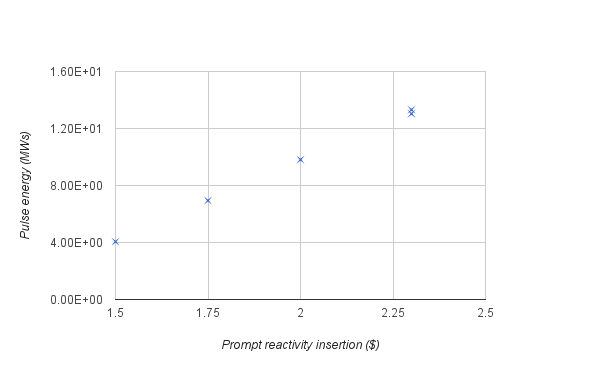
\includegraphics[height=0.4\textheight]{figa/energy.png}
	\mycaption[Pulse energy as a function of the prompt reactivity inserted]{Pulse energy as a function of the prompt reactivity inserted.}
	\label{fig:energy}
\end{figure}

\begin{figure}[t!]
	\centering
	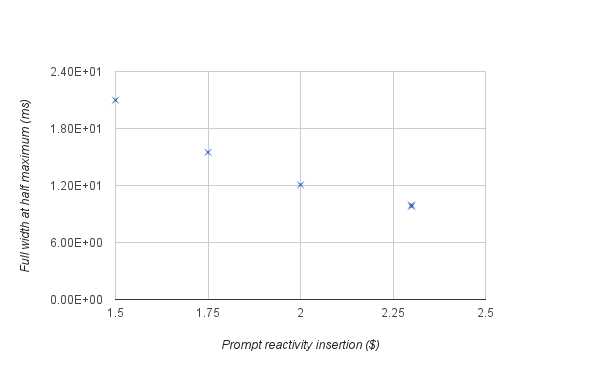
\includegraphics[height=0.4\textheight]{figa/fwhm.png}
	\mycaption[Pulse FWHM as a function of the prompt reactivity inserted]{Pulse FWHM as a function of the prompt reactivity inserted.}
	\label{fig:fwhm}
\end{figure}

\begin{figure}[t!]
	\centering
	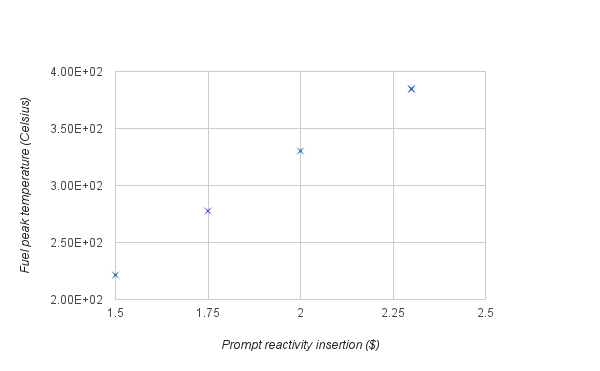
\includegraphics[height=0.4\textheight]{figa/temperature.png}
	\mycaption[Fuel temperature as a function of the prompt reactivity inserted]{Fuel temperature as a function of the prompt reactivity inserted.}
	\label{fig:temperature}
\end{figure}

\begin{figure}[t!]
	\centering
	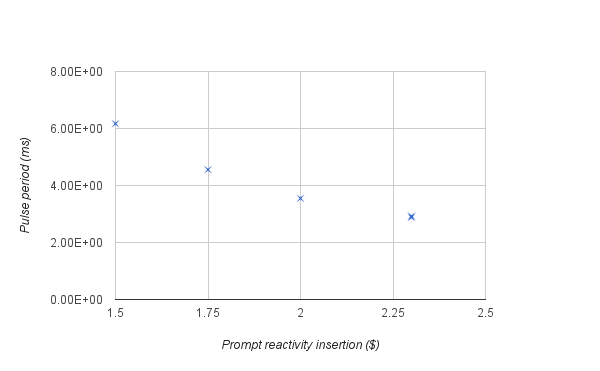
\includegraphics[height=0.4\textheight]{figa/period.png}
	\mycaption[Pulse period as a function of the prompt reactivity inserted]{Pulse period as a function of the prompt reactivity inserted.}
	\label{fig:period}
\end{figure}





\
